\chapter{Perancangan}
\label{chap:perancangan}

Pada bab ini dijelaskan mengenai ....

\section{Struktur Penyimpanan Leksikon}
\label{sec:strukturPenyimpananLeksikon}

Leksikon yang dirancang pada perangkat lunak morphological parser ini akan menyimpan kata dasar dan kata turunan yang valid dalam bahasa Indonesia. Kata dasar secara khusus akan dimuat ke dalam program dalam sebuah struktur data trie supaya dapat diakses dengan cepat dan efektif. Sementara kata turunan akan diakses setelah proses parsing selesai untuk melakukan validasi terhadap hasil dari proses parsing. Kata dasar dan kata turunan tersebut harus disimpan dalam file khusus supaya dapat dimuat dan diakses oleh program ketika program dijalankan.

Semua kata dasar disimpan pada sebuah file yang bernama 'roots' berekstensi '.lxc' pada sebuah folder dalam program. Setiap entri kata dasar dipisahkan oleh karakter enter dan disimpan terurut berdasarkan urutan abjad. Untuk menyimpan kata turunan dari setiap kata dasar, dibuat sebuah file khusus dengan nama file sama dengan kata dasar dan berekstensi '.lxc' yang disimpan pada folder yang sama. Isi dari setiap file tersebut adalah kata dasar diikuti oleh semua kemungkinan kata turunan yang dapat dibentuk dari kata dasar yang bersangkutan.

Penyimpanan kata turunan tidak bisa dilakukan dengan menulis semua bentuk turunan secara langsung karena akan sangat tidak efisien, terutama untuk bentuk turunan dari afiks yang sangat produktif seperti prefiks \textit{ber-} dan prefiks \textit{me-}. Perlu struktur khusus untuk menyimpan semua kata turunan dengan efisien dalam setiap file kata dasar. Oleh karena itu, dirancang beberapa lambang leksikon seperti dapat dilihat pada tabel \ref{tabel-lambang-leksikon} berikut.

\begin{table}[H]
\centering
\begin{tabular}{|c|c|}
\hline
\textbf{Bentuk} & \textbf{Lambang leksikon} \\
\hline
Komposisi&@\\
Reduplikasi&\textasciicircum\\
Prefiks&[\\
Sufiks&]\\
Konfiks&\# ..-..\\
\hline
\end{tabular}
\caption{Tabel Lambang Bentuk Turunan dalam Leksikon} 
\label{tabel-lambang-leksikon}
\end{table}

Untuk menyimpan kata turunan 'sayur bening' yang merupakan hasil proses komposisi dari kata 'sayur' digabung dengan kata 'bening', kita bisa menambahkan bentuk '@bening' dalam file 'sayur.lxc'. Untuk menyimpan kata 'sayur-mayur' yang merupakan hasil reduplikasi berubah bunyi dari kata 'sayur', kita bisa menuliskan bentuk '\textasciicircum mayur'. Sementara untuk bentuk turunan hasil dari proses prefiksasi dan sufiksasi seperti kata 'menyayur' dan 'sayuran', dapat disimpan dalam bentuk '[me' dan ']an'. Untuk kata yang merupakan hasil dari proses konfiksasi seperti kata 'kesatuan', kita bisa menyimpannya dalam file 'satu.lxc' dengan bentuk '\# ke-an'.

Suatu kata turunan dapat dibentuk dari lebih dari satu proses morfologi, misalnya kata 'sayur-sayuran' merupakan kata dasar 'sayur' yang dilakukan reduplikasi utuh menjadi 'sayur-sayur' lalu dibubuhkan sufiks \textit{-an} menjadi bentuk 'sayur-sayuran'. Untuk menyimpan bentuk tersebut, setiap proses dapat dipisahkan dengan simbol '+' dengan proses yang lebih dulu dikerjakan ditulis lebih dahulu. Untuk menyimpan bentuk reduplikasi utuh, kita bisa menyimpannya dengan bentuk '\textasciicircum 2'. Kata turunan 'sayur-sayuran' disimpan dalam file 'sayur.lxc' dengan bentuk '\textasciicircum 2+]an'. Untuk kasus kata yang merupakan hasil dari proses reduplikasi dan afiksasi, penulisan bentuk turunan selalu proses reduplikasi ditulis lebih dahulu baru diikuti oleh proses afiksasi. 

Gambar \ref{contoh-entri-sayur} berikut adalah contoh isi dari file 'sayur.lxc' yang berisi semua kata turunan dari kata dasar 'sayur'.

\begin{figure}[H]
\centering
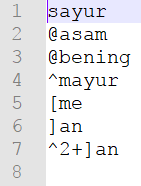
\includegraphics[scale=1]{Gambar/contoh-entri-sayur}
\caption{Isi dari file sayur.lxc} 
\label{contoh-entri-sayur}
\end{figure}

Pada kasus di mana terdapat lebih dari satu prefiks seperti pada kata 'memperkuat', maka prefiks yang lebih dulu dibubuhkan pada kata dasar ditulis terlebih dahulu. Kata 'memperkuat' disimpan dalam file 'kuat.lxc' dengan bentuk '[per+[me'. Sementara untuk kasus pada proses klofiksasi, di mana ada prefiks dan sufiks yang diimbuhkan tetapi pengimbuhannya tidak sekaligus, urutan penulisannya adalah sufiks ditulis lebih dahulu dari prefiks. Contohnya pada kata 'berlarian' disimpan dalam file 'lari.lxc' dalam bentuk ']an+[ber'.

Pada kasus kata yang merupakan hasil dari proses komposisi dan prefiksasi, seperti pada kata 'bekerja bakti', proses yang lebih dulu ditulis adalah proses yang melekat pada kata dasarnya yaitu proses prefiksasi \textit{ber-} pada kata 'kerja'. Kata 'bekerja bakti' disimpan dalam file 'kerja.lxc' dengan bentuk '[ber+@bakti'. Sementara pada contoh kasus kata yang merupakan hasil dari proses komposisi dan konfiksasi, seperti pada kata 'pertanggungjawaban', proses yang lebih dulu ditulis adalah proses komposisi kata 'tanggung' dengan kata 'jawab'. Kata 'pertanggungjawaban' disimpan dalam file 'tanggung.lxc' dengan bentuk '@jawab+\# per-an'. Hal ini berlaku juga untuk kata yang merupakan hasil dari proses komposisi dan klofiksasi, seperti pada kata 'menanggungjawabi' yang disimpan dengan bentuk '@jawab+]i+[me'.


\section{Syntax Keluaran Proses Morphological Parsing}
\label{sec:syntaxKeluaran}

Pada subbab \ref{sec:morfem} disebutkan bahwa dalam konvensi linguistik sebuah bentuk dinyatakan sebagai morfem ditulis dalam kurung kurawal ($\lbrace$...$\rbrace$). Proses morphological parsing merupakan proses memisahkan sebuah kata menjadi morfem-morfem penyusunnya. Oleh karena itu, keluaran dari proses morphological parsing sebaiknya mengikuti konvensi linguistik di mana setiap morfem penyusun kata ditulis dalam kurung kurawal ($\lbrace$...$\rbrace$).

Morfem penyusun kata dalam proses morfologi dapat terdiri dari beberapa jenis, yaitu morfem dasar dan morfem afiks dalam proses afiksasi, morfem dasar dengan dirinya sendiri dalam proses reduplikasi, dan morfem dasar dengan morfem dasar lain dalam proses komposisi. Morfem afiks dibagi menjadi tiga jenis, yaitu prefiks, sufiks, dan konfiks. 

Proses morphological parsing yang dirancang pada penelitian ini akan menghasilkan keluaran berupa bentuk dasar diikuti oleh proses morfologi yang dilakukan kepada bentuk dasar tersebut. Sebagai contoh, jika masukan adalah kata 'pertanggungjawaban' maka keluaran dari proses morphological parsing terhadap kata tersebut adalah bentuk dasar $\lbrace$tanggung$\rbrace$ diikuti proses komposisi $\lbrace$jawab$\rbrace$ lalu diikuti proses konfiksasi $\lbrace$per-an$\rbrace$. Untuk menyederhanakan keluaran, kata 'proses' tidak ditulis, kata 'diikuti' diganti dengan simbol '+', dan proses seperti 'konfiksasi' hanya ditulis 'konfiks' saja, sehingga keluaran dari proses tersebut menjadi bentuk dasar $\lbrace$tanggung$\rbrace$ + komposisi $\lbrace$jawab$\rbrace$ + konfiks $\lbrace$per-an$\rbrace$. Untuk kata yang merupakan hasil reduplikasi, seperti kata 'buah-buahan', hasil proses parsing terhadap kata tersebut adalah bentuk dasar $\lbrace$buah$\rbrace$ + reduplikasi $\lbrace$2$\rbrace$ + sufiks $\lbrace$an$\rbrace$. Bentuk '2' dalam reduplikasi berarti reduplikasi utuh.

Seperti dijelaskan pada subbab \ref{sec:leksikon}, leksikon menyimpan setiap kata turunan yang valid dari sebuah kata dasar supaya perangkat lunak dapat melakukan validasi terhadap hasil dari proses parsing. Oleh karena itu, keluaran dari proses parsing harus menggunakan simbol yang sama dengan leksikon supaya hasil dari proses parsing dapat dibandingkan dengan kata turunan yang disimpan dalam leksikon untuk melakukan validasi. Dengan menggunakan simbol pada tabel \ref{tabel-lambang-leksikon}, keluaran dari proses parsing terhadap kata 'pertanggungjawaban' adalah bentuk dasar 'tanggung' ditambah proses morfologi '@jawab+\# per-an'. Dengan demikian, perangkat lunak dapat melakukan validasi terhadap bentuk '@jawab+\# per-an' apakah merupakan bentuk turunan yang valid atau tidak dari kata 'tanggung' dalam leksikon.

Berdasarkan penjelasan di atas, dapat disimpulkan ada dua jenis keluaran dari proses morphological parsing, yaitu keluaran dalam bentuk simbol seperti dalam leksikon dan keluaran dalam bentuk kata-kata yang dapat dimengerti oleh manusia. Perangkat lunak pertama kali membuat keluaran dalam bentuk simbol yang kemudian divalidasi oleh leksikon. Keluaran yang dianggap tidak valid akan dibuang oleh perangkat lunak sementara keluaran yang dianggap valid kemudian diterjemahkan menjadi keluaran berupa kata-kata yang dimengerti oleh manusia.

\section{Perancangan Antarmuka}
\label{sec:perancanganAntarmuka}

Antarmuka yang akan dibuat terdiri dari dua jenis, yaitu untuk perangkat lunak morphological parser dan perangkat lunak lexicon. Sesuai use case yang diuraikan pada subbab \ref{sec:AnalisisUseCase}, perangkat lunak lexicon memiliki dua jenis user, yaitu user biasa dan editor. Antarmuka untuk perangkat lunak morphological parser terdiri dari sebuah \textit{frame} sementara untuk perangkat lunak lexicon terdiri dari enam buah \textit{frame} yang masing-masing mewakili sebuah fitur untuk sebuah user dari perangkat lunak. Berikut adalah penjelasan untuk setiap rancangan antarmuka yang dibuat.

\subsection{Perancangan Antarmuka Perangkat Lunak Morphological Parser}
\label{sec:antarmukaParser}

Gambar \ref{mockup-parser} berikut adalah rancangan antarmuka yang dibuat untuk perangkat lunak morphological parser.

\begin{figure}[H]
\centering
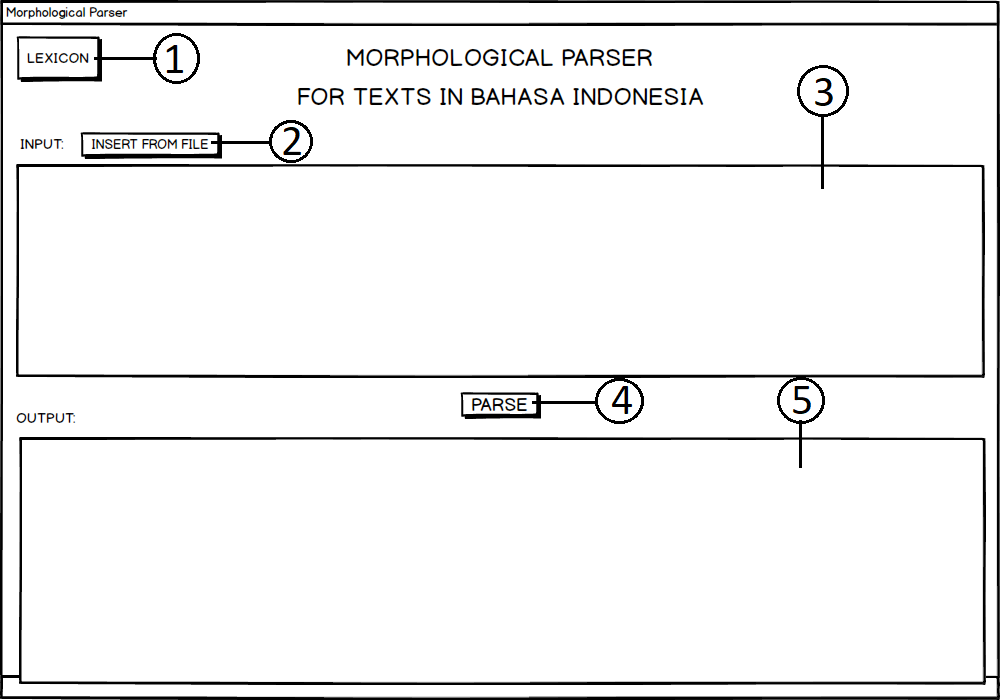
\includegraphics[scale=0.7]{Gambar/mockup-parser}
\caption{Rancangan antarmuka perangkat lunak morphological parser} 
\label{mockup-parser}
\end{figure}

Penjelasan untuk setiap objek dalam \textit{frame} di atas adalah sebagai berikut.

\begin{enumerate}
	\item Tombol \textit{Lexicon}: untuk mengakses perangkat lunak lexicon
	\item Tombol \textit{Insert From File}: untuk memuat isi dari sebuah file txt ke dalam kolom masukan dari perangkat lunak
	\item Kolom masukan: untuk menulis masukan dari proses parsing
	\item Tombol \textit{Parse}: untuk melakukan proses parsing terhadap teks dalam kolom masukan dan mengeluarkan hasilnya pada kolom keluaran
	\item Kolom keluaran: untuk menampilkan keluaran dari proses parsing
\end{enumerate}

\subsection{Perancangan Antarmuka Perangkat Lunak Lexicon}
\label{sec:antarmukaLexicon}

Gambar \ref{mockup-lexicon-home-user} berikut adalah rancangan antarmuka yang dibuat untuk perangkat lunak lexicon pada halaman home untuk user.

\begin{figure}[H]
\centering
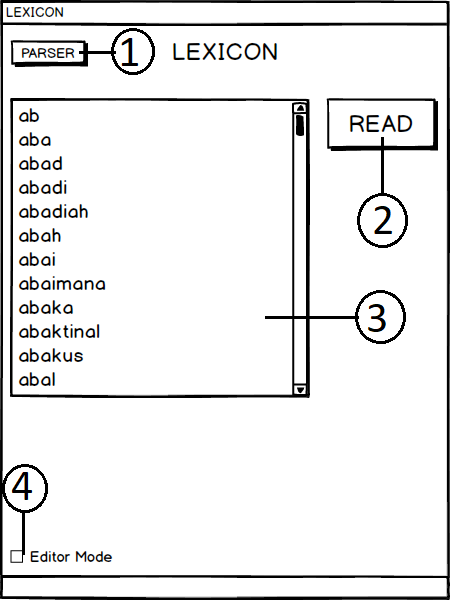
\includegraphics[scale=0.8]{Gambar/mockup-lexicon-home-user}
\caption{Rancangan antarmuka perangkat lunak lexicon halaman home untuk user} 
\label{mockup-lexicon-home-user}
\end{figure}

Penjelasan untuk setiap objek dalam \textit{frame} di atas adalah sebagai berikut.

\begin{enumerate}
	\item Tombol \textit{Parser}: untuk mengakses perangkat lunak morphological parser
	\item Tombol \textit{Read}: untuk melihat kata turunan dari sebuah entri kata dasar pada leksikon
	\item Kolom entri leksikon: untuk menampilkan semua entri kata dasar yang disimpan dalam leksikon
	\item Tombol \textit{Editor mode}: untuk mengaktifkan atau mematikan mode editor pada perangkat lunak lexicon
\end{enumerate}

Gambar \ref{mockup-lexicon-read-user} berikut adalah rancangan antarmuka yang dibuat untuk perangkat lunak lexicon pada halaman read untuk user.

\begin{figure}[H]
\centering
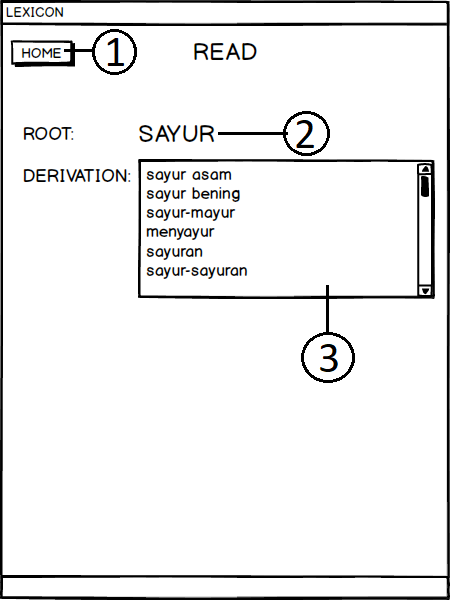
\includegraphics[scale=0.8]{Gambar/mockup-lexicon-read-user}
\caption{Rancangan antarmuka perangkat lunak lexicon halaman read untuk user} 
\label{mockup-lexicon-read-user}
\end{figure}

Penjelasan untuk setiap objek dalam \textit{frame} di atas adalah sebagai berikut.

\begin{enumerate}
	\item Tombol \textit{Home}: untuk kembali ke halaman home dari perangkat lunak lexicon
	\item Label root: untuk menampilkan kata dasar yang sedang dilihat saat ini
	\item Kolom entri kata turunan: untuk menampilkan semua entri kata turunan dari kata dasar yang disimpan dalam leksikon
\end{enumerate}

Gambar \ref{mockup-lexicon-home-editor} berikut adalah rancangan antarmuka yang dibuat untuk perangkat lunak lexicon pada halaman home untuk editor.

\begin{figure}[H]
\centering
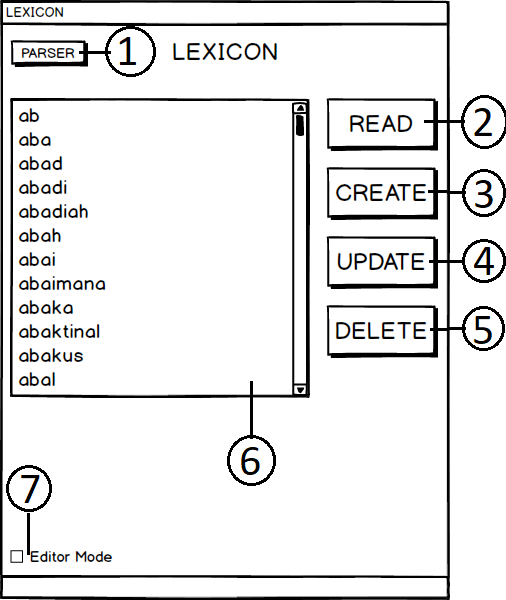
\includegraphics[scale=0.8]{Gambar/mockup-lexicon-home-editor}
\caption{Rancangan antarmuka perangkat lunak lexicon halaman home untuk editor} 
\label{mockup-lexicon-home-editor}
\end{figure}

Penjelasan untuk setiap objek dalam \textit{frame} di atas adalah sebagai berikut.

\begin{enumerate}
	\item Tombol \textit{Parser}: untuk mengakses perangkat lunak morphological parser
	\item Tombol \textit{Read}: untuk melihat kata turunan dari sebuah entri kata dasar pada leksikon
	\item Tombol \textit{Create}: untuk memasukkan entri baru pada leksikon
	\item Tombol \textit{Update}: untuk mengubah entri pada leksikon
	\item Tombol \textit{Delete}: untuk menghapus entri pada leksikon
	\item Kolom entri leksikon: untuk menampilkan semua entri kata dasar yang disimpan dalam leksikon
	\item Tombol \textit{Editor mode}: untuk mengaktifkan atau mematikan mode editor pada perangkat lunak lexicon
\end{enumerate}

Gambar \ref{mockup-lexicon-create-editor} berikut adalah rancangan antarmuka yang dibuat untuk perangkat lunak lexicon pada halaman create untuk editor.

\begin{figure}[H]
\centering
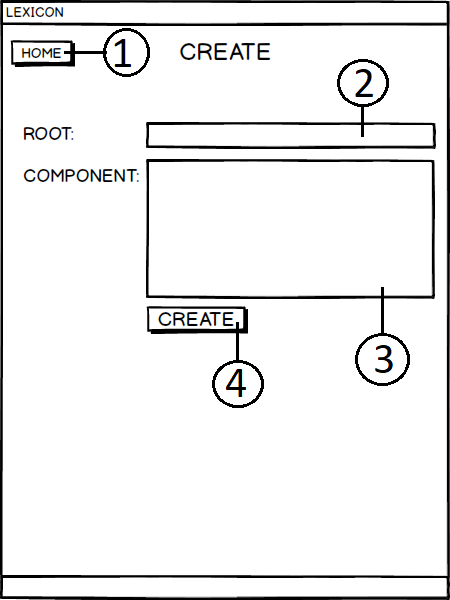
\includegraphics[scale=0.8]{Gambar/mockup-lexicon-create-editor}
\caption{Rancangan antarmuka perangkat lunak lexicon halaman create untuk editor} 
\label{mockup-lexicon-create-editor}
\end{figure}

Penjelasan untuk setiap objek dalam \textit{frame} di atas adalah sebagai berikut.

\begin{enumerate}
	\item Tombol \textit{Home}: untuk kembali ke halaman home dari perangkat lunak lexicon
	\item Kolom kata dasar: untuk memasukkan kata dasar dari entri yang akan dibuat
	\item Kolom kata turunan: untuk memasukkan kata turunan dari entri yang akan dibuat
	\item Tombol \textit{Create}: untuk memasukkan entri baru yang sudah dibuat ke dalam leksikon
\end{enumerate}

Gambar \ref{mockup-lexicon-update-editor} berikut adalah rancangan antarmuka yang dibuat untuk perangkat lunak lexicon pada halaman update untuk editor.

\begin{figure}[H]
\centering
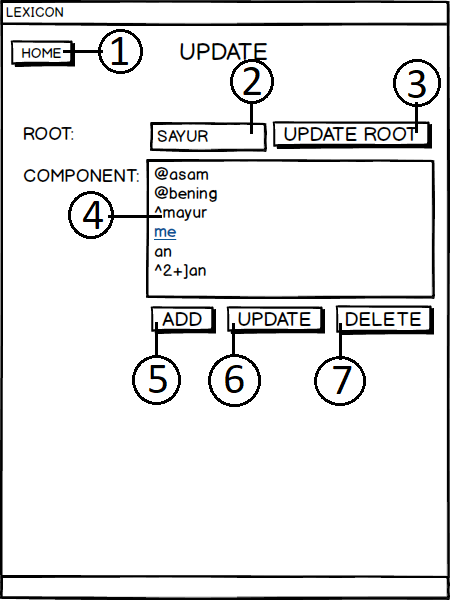
\includegraphics[scale=0.8]{Gambar/mockup-lexicon-update-editor}
\caption{Rancangan antarmuka perangkat lunak lexicon halaman update untuk editor} 
\label{mockup-lexicon-update-editor}
\end{figure}

Penjelasan untuk setiap objek dalam \textit{frame} di atas adalah sebagai berikut.

\begin{enumerate}
	\item Tombol \textit{Home}: untuk kembali ke halaman home dari perangkat lunak lexicon
	\item Kolom kata dasar: untuk mengubah kata dasar dari entri
	\item Tombol \textit{Update Root}: untuk memasukkan entri kata dasar baru ke dalam leksikon
	\item Kolom kata turunan: untuk mengubah kata turunan dari entri
	\item Tombol \textit{Add}: untuk menambahkan entri kata turunan baru pada kata dasar
	\item Tombol \textit{Update}: untuk mengubah entri kata turunan pada kata dasar
	\item Tombol \textit{Delete}: untuk menghapus entri kata turunan pada kata dasar
\end{enumerate}

Gambar \ref{mockup-lexicon-delete-editor} berikut adalah rancangan antarmuka yang dibuat untuk perangkat lunak lexicon pada halaman delete untuk editor.

\begin{figure}[H]
\centering
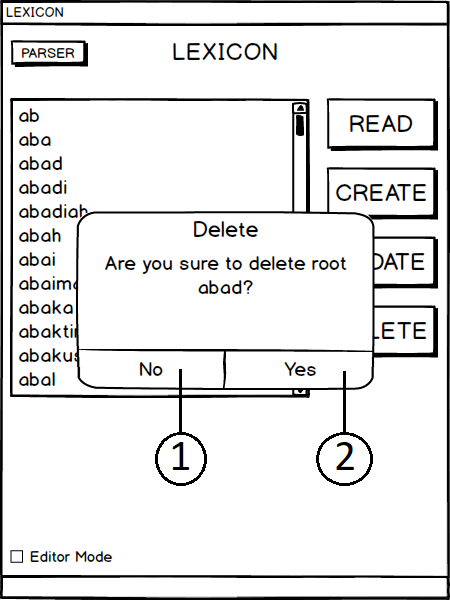
\includegraphics[scale=0.8]{Gambar/mockup-lexicon-delete-editor}
\caption{Rancangan antarmuka perangkat lunak lexicon halaman delete untuk editor} 
\label{mockup-lexicon-delete-editor}
\end{figure}

Penjelasan untuk setiap objek dalam \textit{frame} di atas adalah sebagai berikut.

\begin{enumerate}
	\item Tombol \textit{No}: untuk membatalkan penghapusan entri kata dasar dari leksikon
	\item Tombol \textit{Yes}: untuk melakukan konfirmasi penghapusan entri kata dasar dari leksikon
\end{enumerate}


\section{Diagram Kelas Lengkap}
\label{sec:DiagramKelasLengkap}

Pada subbab \ref{sec:DiagramKelasAwal} telah diuraikan analisis mengenai kelas-kelas yang akan dibuat untuk perangkat lunak morphological parser. Pada subbab ini akan ditambahkan beberapa kelas dan method untuk melengkapi kelas-kelas yang sudah diuraikan sebelumnya. Gambar \ref{gambar-diagram-kelas-final} adalah diagram kelas lengkap yang dibuat untuk perangkat lunak morphological parser.

\begin{figure}[H]
\centering
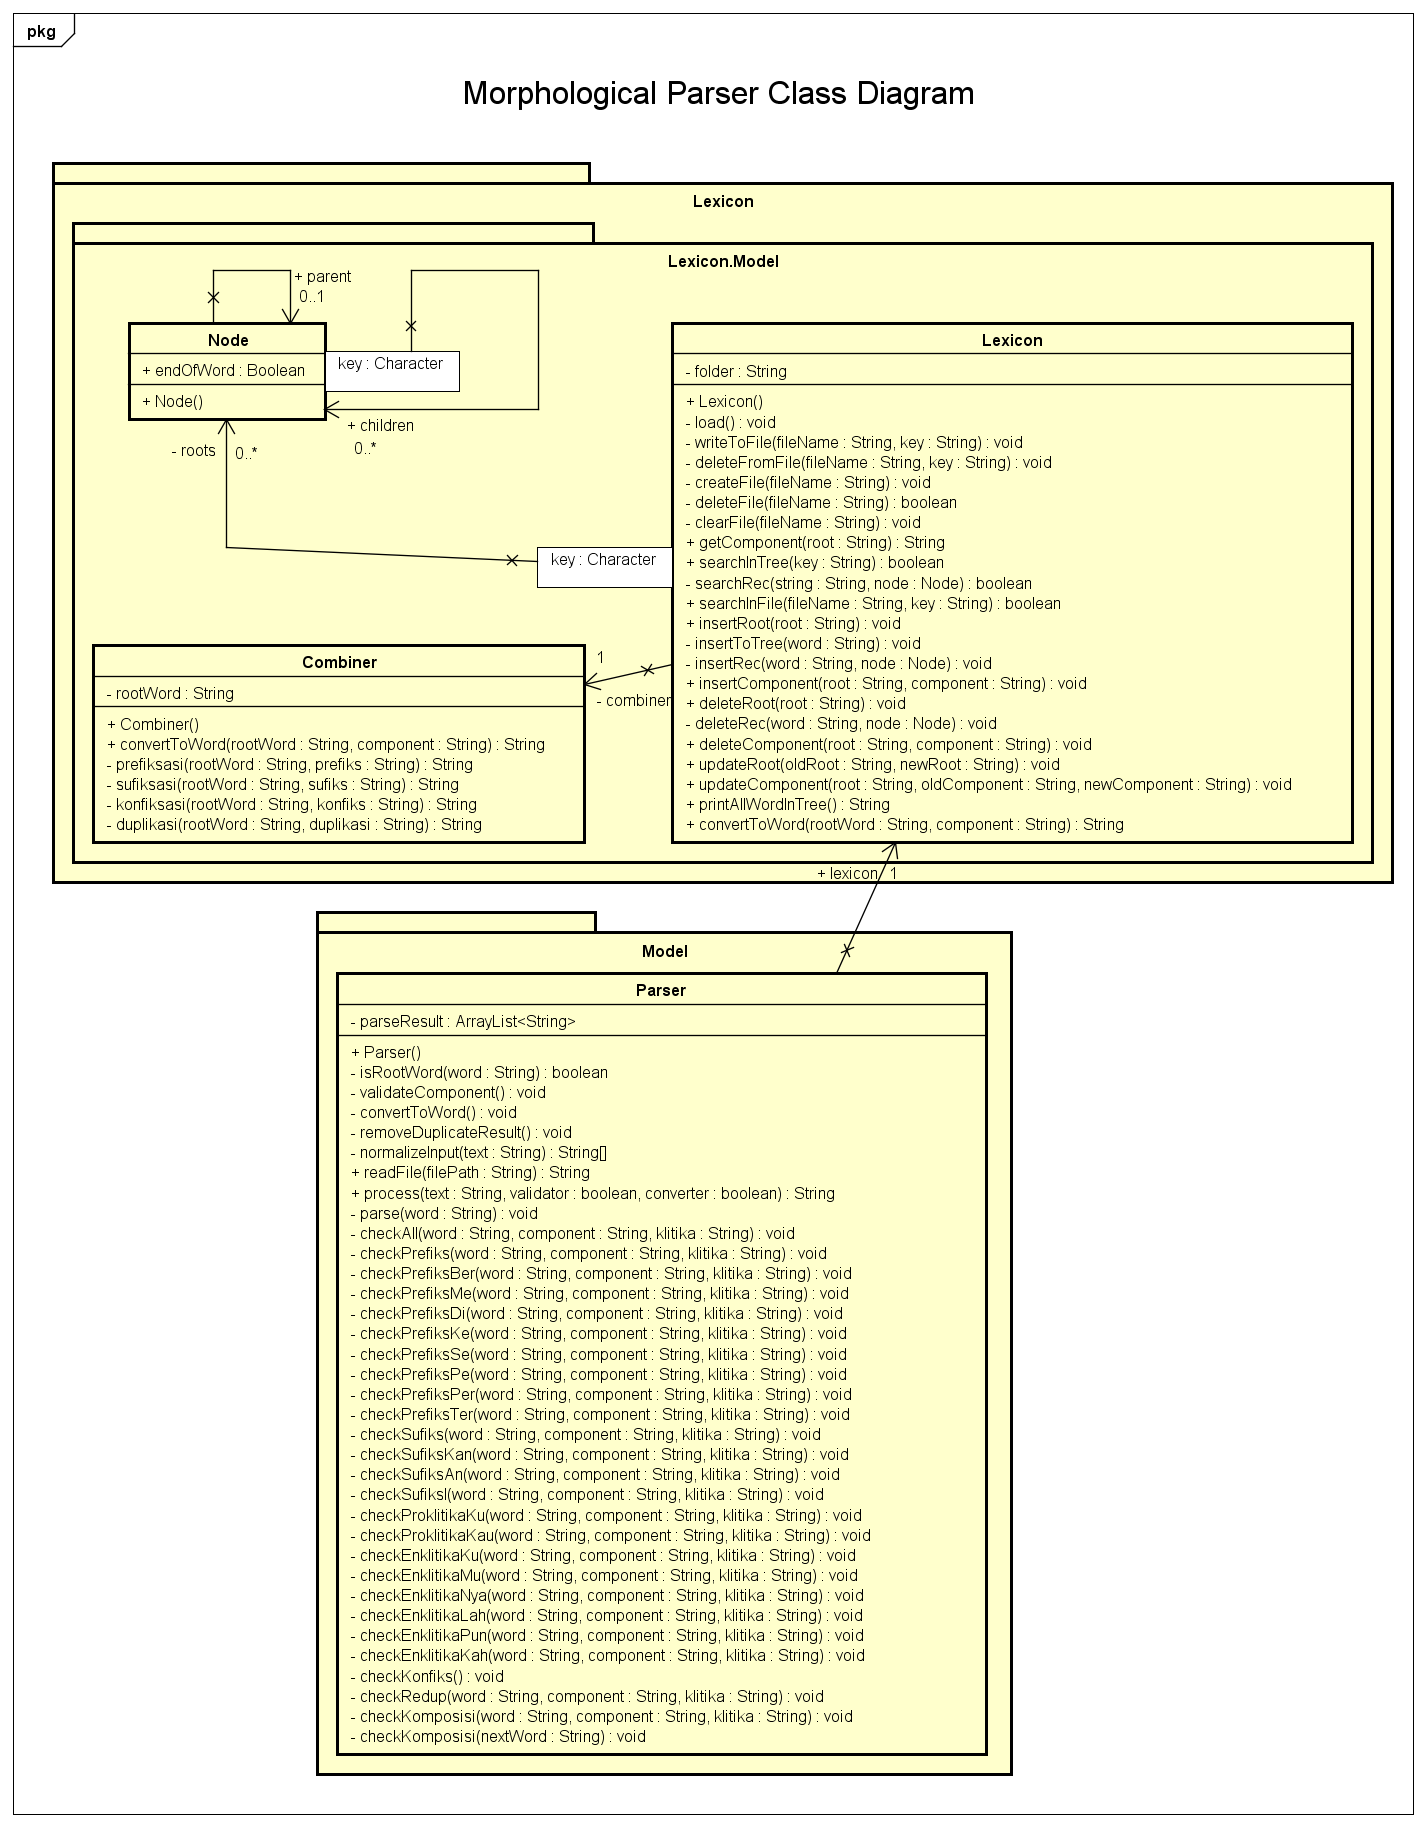
\includegraphics[scale=0.4]{Gambar/gambar-diagram-kelas-final}
\caption{Diagram kelas lengkap perangkat lunak morphological parser} 
\label{gambar-diagram-kelas-final}
\end{figure}

\subsection{Kelas Parser}
\label{sec:kelasParser}

Kelas ini berfungsi untuk melakukan proses parsing terhadap sebuah kalimat atau paragraf dalam bahasa Indonesia.

Atribut yang terdapat dalam kelas ini adalah:

\begin{itemize}
	\item \textit{parseResult}: bertipe ArrayList of String untuk menyimpan beberapa kemungkinan hasil parsing dari setiap kata dalam kalimat atau paragraf yang menjadi masukan
	\item \textit{lexicon}: bertipe objek dari kelas Lexicon dan merupakan objek yang digunakan oleh kelas Parser untuk mengakses fitur leksikon dari perangkat lunak
\end{itemize}

Method yang terdapat dalam kelas ini adalah:

\begin{itemize}
	\item \textit{Parser}: konstruktor tanpa parameter untuk membuat objek dari kelas Parser.
	\item \textit{isRootWord}: method dengan sebuah parameter bertipe String dan kembalian bertipe boolean untuk menentukan apakah kata yang ada di parameter merupakan kata dasar atau bukan. Method ini memanggil method searchInTree dari kelas Lexicon.
	\item \textit{validateComponent}: method tanpa parameter dan kembalian bertipe void untuk melakukan validasi terhadap hasil parsing dengan melakukan pengecekan kata turunan dalam leksikon.
	\item \textit{convertToWord}: method tanpa parameter dan kembalian bertipe void untuk melakukan konversi hasil parsing dari simbol leksikon ke kata-kata yang dapat dimengerti oleh manusia.
	\item \textit{removeDuplicateResult}: method tanpa parameter dan kembalian bertipe void untuk menghapus hasil parsing yang memiliki duplikat pada atribut hasil parsing.
	\item \textit{normalizeInput}: method dengan sebuah parameter bertipe String dan kembalian bertipe array of String untuk melakukan normalisasi pada teks pada parameter dengan membuat semua karakter huruf menjadi huruf kecil, membuang karakter yang tidak diperlukan, dan memisahkan teks berdasar karakter spasi. Karakter yang diperlukan adalah karakter huruf kecil (a..z), karakter pemisah (-), dan karakter angka (0..9).
	\item \textit{readFile}: method dengan sebuah parameter bertipe String dan kembalian bertipe String untuk isi file dari path yang ada di parameter dan mengembalikan isinya.
	\item \textit{process}: method dengan sebuah parameter bertipe String, dua buah parameter bertipe boolean, dan kembalian bertipe String untuk melakukan proses parsing terhadap teks yang ada di parameter. Fitur validator dan converter untuk hasil dari proses parsing dapat dinyalakan dan dimatikan bergantung pada nilai dari parameter validator dan converter. 
	\item \textit{parse}: method dengan sebuah parameter bertipe String dan kembalian bertipe void untuk melakukan parsing pada sebuah kata dalam parameter. Hasil parsing disimpan dalam atribut parseResult.
	\item \textit{checkPrefiks}: method dengan tiga buah parameter bertipe String dan kembalian bertipe void untuk melakukan pengecekan ada atau tidak prefiks dalam String kata yang diberikan di parameter. Parameter component dan klitika menyimpan component dan klitika yang sudah ditemukan ketika method ini dipanggil.
	\item \textit{checkSufiks}: method dengan tiga buah parameter bertipe String dan kembalian bertipe void untuk melakukan pengecekan ada atau tidak sufiks dalam String kata yang diberikan di parameter. Parameter component dan klitika menyimpan component dan klitika yang sudah ditemukan ketika method ini dipanggil.
	\item \textit{checkRedup}: method dengan tiga buah parameter bertipe String dan kembalian bertipe void untuk melakukan pengecekan reduplikasi dalam String kata yang diberikan di parameter. Parameter component dan klitika menyimpan component dan klitika yang sudah ditemukan ketika method ini dipanggil.
	\item \textit{check}: method dengan tiga buah parameter bertipe String dan kembalian bertipe void untuk melakukan pengecekan terhadap semua kemungkinan proses morfologi dalam String kata yang diberikan di parameter. Parameter component dan klitika menyimpan component dan klitika yang sudah ditemukan ketika method ini dipanggil.
	\item \textit{prefiksBer}: method dengan tiga buah parameter bertipe String dan kembalian bertipe void untuk melakukan pengecekan ada atau tidak prefiks ber- dalam String kata yang diberikan di parameter. Parameter component dan klitika menyimpan component dan klitika yang sudah ditemukan ketika method ini dipanggil.
	\item \textit{prefiksMe}: method dengan tiga buah parameter bertipe String dan kembalian bertipe void untuk melakukan pengecekan ada atau tidak prefiks me- dalam String kata yang diberikan di parameter. Parameter component dan klitika menyimpan component dan klitika yang sudah ditemukan ketika method ini dipanggil.
	\item \textit{prefiksDi}: method dengan tiga buah parameter bertipe String dan kembalian bertipe void untuk melakukan pengecekan ada atau tidak prefiks di- dalam String kata yang diberikan di parameter. Parameter component dan klitika menyimpan component dan klitika yang sudah ditemukan ketika method ini dipanggil.
	\item \textit{prefiksKe}: method dengan tiga buah parameter bertipe String dan kembalian bertipe void untuk melakukan pengecekan ada atau tidak prefiks ke- dalam String kata yang diberikan di parameter. Parameter component dan klitika menyimpan component dan klitika yang sudah ditemukan ketika method ini dipanggil.
	\item \textit{proklitikaKu}: method dengan tiga buah parameter bertipe String dan kembalian bertipe void untuk melakukan pengecekan ada atau tidak proklitika ku- dalam String kata yang diberikan di parameter. Parameter component dan klitika menyimpan component dan klitika yang sudah ditemukan ketika method ini dipanggil.
	\item \textit{prefiksSe}: method dengan tiga buah parameter bertipe String dan kembalian bertipe void untuk melakukan pengecekan ada atau tidak prefiks se- dalam String kata yang diberikan di parameter. Parameter component dan klitika menyimpan component dan klitika yang sudah ditemukan ketika method ini dipanggil.
	\item \textit{prefiksPe}: method dengan tiga buah parameter bertipe String dan kembalian bertipe void untuk melakukan pengecekan ada atau tidak prefiks pe- dalam String kata yang diberikan di parameter. Parameter component dan klitika menyimpan component dan klitika yang sudah ditemukan ketika method ini dipanggil.
	\item \textit{prefiksPer}: method dengan tiga buah parameter bertipe String dan kembalian bertipe void untuk melakukan pengecekan ada atau tidak prefiks per- dalam String kata yang diberikan di parameter. Parameter component dan klitika menyimpan component dan klitika yang sudah ditemukan ketika method ini dipanggil.
	\item \textit{prefiksTer}: method dengan tiga buah parameter bertipe String dan kembalian bertipe void untuk melakukan pengecekan ada atau tidak prefiks ter- dalam String kata yang diberikan di parameter. Parameter component dan klitika menyimpan component dan klitika yang sudah ditemukan ketika method ini dipanggil.
	\item \textit{proklitikaKau}: method dengan tiga buah parameter bertipe String dan kembalian bertipe void untuk melakukan pengecekan ada atau tidak proklitika kau- dalam String kata yang diberikan di parameter. Parameter component dan klitika menyimpan component dan klitika yang sudah ditemukan ketika method ini dipanggil.
	\item \textit{sufiksKan}: method dengan tiga buah parameter bertipe String dan kembalian bertipe void untuk melakukan pengecekan ada atau tidak sufiks -kan dalam String kata yang diberikan di parameter. Parameter component dan klitika menyimpan component dan klitika yang sudah ditemukan ketika method ini dipanggil.
	\item \textit{sufiksAn}: method dengan tiga buah parameter bertipe String dan kembalian bertipe void untuk melakukan pengecekan ada atau tidak sufiks -an dalam String kata yang diberikan di parameter. Parameter component dan klitika menyimpan component dan klitika yang sudah ditemukan ketika method ini dipanggil.
	\item \textit{sufiksI}: method dengan tiga buah parameter bertipe String dan kembalian bertipe void untuk melakukan pengecekan ada atau tidak sufiks -i dalam String kata yang diberikan di parameter. Parameter component dan klitika menyimpan component dan klitika yang sudah ditemukan ketika method ini dipanggil.
	\item \textit{enklitikaKu}: method dengan tiga buah parameter bertipe String dan kembalian bertipe void untuk melakukan pengecekan ada atau tidak enklitika -ku dalam String kata yang diberikan di parameter. Parameter component dan klitika menyimpan component dan klitika yang sudah ditemukan ketika method ini dipanggil.
	\item \textit{enklitikaMu}: method dengan tiga buah parameter bertipe String dan kembalian bertipe void untuk melakukan pengecekan ada atau tidak enklitika -mu dalam String kata yang diberikan di parameter. Parameter component dan klitika menyimpan component dan klitika yang sudah ditemukan ketika method ini dipanggil.
	\item \textit{enklitikaNya}: method dengan tiga buah parameter bertipe String dan kembalian bertipe void untuk melakukan pengecekan ada atau tidak enklitika -nya dalam String kata yang diberikan di parameter. Parameter component dan klitika menyimpan component dan klitika yang sudah ditemukan ketika method ini dipanggil.
	\item \textit{enklitikaLah}: method dengan tiga buah parameter bertipe String dan kembalian bertipe void untuk melakukan pengecekan ada atau tidak enklitika -lah dalam String kata yang diberikan di parameter. Parameter component dan klitika menyimpan component dan klitika yang sudah ditemukan ketika method ini dipanggil.
	\item \textit{enklitikaPun}: method dengan tiga buah parameter bertipe String dan kembalian bertipe void untuk melakukan pengecekan ada atau tidak enklitika -pun dalam String kata yang diberikan di parameter. Parameter component dan klitika menyimpan component dan klitika yang sudah ditemukan ketika method ini dipanggil.
	\item \textit{enklitikaKah}: method dengan tiga buah parameter bertipe String dan kembalian bertipe void untuk melakukan pengecekan ada atau tidak enklitika -kah dalam String kata yang diberikan di parameter. Parameter component dan klitika menyimpan component dan klitika yang sudah ditemukan ketika method ini dipanggil.
	\item \textit{checkKonfiks}: method tanpa parameter dan kembalian bertipe void untuk melakukan pengecekan adanya kemungkinan kombinasi prefiks dan sufiks yang membentuk konfiks pada atribut hasil parsing.
	\item \textit{checkKomposisi}: method dengan tiga buah parameter bertipe String dan kembalian bertipe void untuk melakukan pengecekan komposisi dalam String kata yang diberikan di parameter. Parameter component dan klitika menyimpan component dan klitika yang sudah ditemukan ketika method ini dipanggil.
	\item \textit{checkKomposisi}: method dengan sebuah parameter bertipe String dan kembalian bertipe void untuk melakukan pengecekan kemungkinan komposisi antara kata yang sedang diproses dengan String kata yang diberikan di parameter.
\end{itemize}

\subsection{Kelas Lexicon}
\label{sec:kelasLexicon}

Kelas ini berfungsi untuk menyimpan kumpulan kata dasar dan kata turunan yang digunakan selama proses morphological parsing berlangsung. Seperti telah diuraikan pada subbab \ref{sec:strukturPenyimpananLeksikon}, kata dasar disimpan dalam sebuah file bernama 'roots.lxc' dan kata turunan untuk setiap kata dasar disimpan dalam file bernama sama dengan kata dasar yang bersangkutan. File 'roots.lxc' akan dimuat oleh kelas ini setiap kali program dijalankan dan kata dasar akan disimpan dalam trie yang berbentuk pohon node supaya pencarian kata dasar dapat dilakukan dengan cepat dan efektif.

Atribut yang terdapat dalam kelas ini adalah:

\begin{itemize}
	\item \textit{roots}: bertipe map of Node dengan key adalah sebuah karakter dan menyimpan kumpulan akar dari pohon node yang menyimpan kata dasar yang valid dalam bahasa Indonesia
	\item \textit{folder}: bertipe String dan menyimpan path dari folder tempat file leksikon berada
\end{itemize}

Method yang terdapat dalam kelas ini adalah:

\begin{itemize}
	\item \textit{Lexicon}: konstruktor tanpa parameter untuk membuat objek dari kelas Lexicon.
	\item \textit{load}: method tanpa parameter dan kembalian bertipe void untuk memuat semua kata dasar dalam leksikon dan menyimpannya ke dalam trie.
	\item \textit{writeToFile}: method dengan dua buah parameter bertipe String dan kembalian bertipe void untuk menulis parameter key ke dalam file dengan nama file dalam parameter fileName.
	\item \textit{deleteFromFile}: method dengan dua buah parameter bertipe String dan kembalian bertipe void untuk menghapus parameter key dari dalam file dengan nama file dalam parameter fileName.
	\item \textit{createFile}: method dengan sebuah parameter bertipe String dan kembalian bertipe void untuk membuat sebuah file baru dengan nama file dalam parameter fileName.
	\item \textit{deleteFile}: method dengan sebuah parameter bertipe String dan kembalian bertipe boolean untuk menghapus sebuah file dengan nama file dalam parameter fileName dan mengembalikan status keberhasilan penghapusan file.
	\item \textit{clearFile}: method dengan sebuah parameter bertipe String dan kembalian bertipe void untuk mengosongkan isi sebuah file dengan nama file dalam parameter fileName.
	\item \textit{getComponent}: method dengan sebuah parameter bertipe String dan kembalian bertipe String untuk mengembalikan semua komponen kata turunan dari sebuah kata dasar dalam parameter root.
	\item \textit{searchInTree}: method dengan sebuah parameter bertipe String dan kembalian bertipe boolean untuk mencari ada atau tidak kata dasar pada parameter key dalam pohon Node.
	\item \textit{searchRec}: method dengan sebuah parameter bertipe String, sebuah parameter bertipe objek dari kelas Node, dan kembalian bertipe boolean untuk melakukan pencarian secara rekursif dalam pohon Node dengan parameter string adalah kata yang dicari dan node adalah node yang sedang ditelusuri saat ini.
	\item \textit{searchInFile}: method dengan dua buah parameter bertipe String dan kembalian bertipe boolean untuk melakukan pencarian dari parameter key dalam file dengan nama pada parameter fileName.
	\item \textit{insertRoot}: method dengan sebuah parameter bertipe String dan kembalian bertipe void untuk memasukkan kata dasar baru dalam parameter root ke dalam leksikon.
	\item \textit{insertToTree}: method dengan sebuah parameter bertipe String dan kembalian bertipe void untuk memasukkan sebuah kata dalam parameter word ke dalam pohon Node.
	\item \textit{insertRec}: method dengan sebuah parameter bertipe String, sebuah parameter bertipe objek dari kelas Node, dan kembalian bertipe void untuk memasukkan kata secara rekursif dalam pohon Node dengan parameter string adalah kata yang dimasukkan dan node adalah node yang sedang ditelusuri saat ini.
	\item \textit{insertComponent}: method dengan dua buah parameter bertipe String dan kembalian bertipe void untuk memasukkan sebuah kata turunan baru dalam parameter component ke kata dasar dalam parameter root.
	\item \textit{deleteRoot}: method dengan sebuah parameter bertipe String dan kembalian bertipe void untuk menghapus sebuah kata dasar dalam parameter root dari pohon Node.
	\item \textit{deleteRec}: method dengan sebuah parameter bertipe String, sebuah parameter bertipe objek dari kelas Node, dan kembalian bertipe void untuk menghapus kata secara rekursif dalam pohon Node dengan parameter string adalah kata yang dihapus dan node adalah node yang sedang ditelusuri saat ini.
	\item \textit{deleteComponent}: method dengan dua buah parameter bertipe String dan kembalian bertipe void untuk menghapus sebuah kata turunan dalam parameter component dari kata dasar dalam parameter root.
	\item \textit{updateRoot}: method dengan dua buah parameter bertipe String dan kembalian bertipe void untuk mengubah kata dasar lama dalam parameter oldRoot menjadi kata dasar baru dalam parameter newRoot.
	\item \textit{updateComponent}: method dengan tiga buah parameter bertipe String dan kembalian bertipe void untuk mengubah kata turunan lama dalam parameter oldComponent menjadi kata turunan baru dalam parameter newComponent untuk kata dasar dalam parameter root.
	\item \textit{printAllWordInTree}: method tanpa parameter dan kembalian bertipe String untuk mencetak semua kata yang disimpan dalam pohon Node ke dalam sebuah String.
	\item \textit{convertToWord}: method dengan dua buah parameter bertipe String dan kembalian bertipe String untuk mengubah kata dasar dalam parameter rootWord dan komponen dalam parameter component menjadi kata-kata yang dapat dimengerti oleh manusia. Method ini memanggil method convertToWord dari kelas Combiner.
\end{itemize}

\subsection{Kelas Node}
\label{sec:kelasNode}

Kelas ini berfungsi untuk merepresentasikan satu node dalam pohon Node.

Atribut yang terdapat dalam kelas ini adalah:

\begin{itemize}
	\item \textit{endOfWord}: bertipe boolean dan menyimpan keterangan apakah node ini merupakan karakter akhir dari sebuah kata dalam pohon atau tidak
	\item \textit{children}: bertipe map of Node dengan key adalah sebuah karakter dan menyimpan kumpulan node yang merupakan anak dari node ini
	\item \textit{parent}: bertipe node dan menyimpan sebuah node yang merupakan parent dari node ini
\end{itemize}

Method yang terdapat dalam kelas ini adalah:

\begin{itemize}
	\item \textit{Node}: konstruktor tanpa parameter untuk membuat objek dari kelas Node.
\end{itemize}

\subsection{Kelas Combiner}
\label{sec:kelasCombiner}

Kelas ini berfungsi untuk melakukan konversi sebuah kata turunan yang disimpan dalam leksikon dari bentuk dalam simbol leksikon menjadi kata yang dapat dimengerti oleh manusia. Ini berfungsi supaya user dari program dapat melihat kata turunan yang disimpan dalam leksikon dalam bentuk kata yang dapat dimengerti dan bukan dalam bentuk simbol leksikon. Kelas ini digunakan dalam fitur Read yang dimiliki oleh perangkat lunak Lexicon.

Atribut yang terdapat dalam kelas ini adalah:

\begin{itemize}
	\item \textit{rootWord}: bertipe String dan menyimpan kata dasar dari kata yang sedang diproses
\end{itemize}

Method yang terdapat dalam kelas ini adalah:

\begin{itemize}
	\item \textit{Combiner}: konstruktor tanpa parameter untuk membuat objek dari kelas Combiner.
	\item \textit{convertToWord}: method dengan dua buah parameter bertipe String dan kembalian bertipe String untuk mengubah kata dasar dalam parameter rootWord dan komponen dalam parameter component menjadi kata-kata yang dapat dimengerti oleh manusia.
	\item \textit{prefiksasi}: method dengan dua buah parameter bertipe String dan kembalian bertipe String untuk melakukan proses prefiksasi pada kata dasar dalam parameter rootWord dan prefiks dalam parameter prefiks.
	\item \textit{sufiksasi}: method dengan dua buah parameter bertipe String dan kembalian bertipe String untuk melakukan proses sufiksasi pada kata dasar dalam parameter rootWord dan sufiks dalam parameter sufiks.
	\item \textit{konfiksasi}: method dengan dua buah parameter bertipe String dan kembalian bertipe String untuk melakukan proses konfiksasi pada kata dasar dalam parameter rootWord dan konfiks dalam parameter konfiks.
	\item \textit{duplikasi}: method dengan dua buah parameter bertipe String dan kembalian bertipe String untuk melakukan proses reduplikasi pada kata dasar dalam parameter rootWord dan jenis reduplikasi dalam parameter duplikasi.
\end{itemize}

\section{Diagram Aktivitas}
\label{sec:diagramAktivitas}

Untuk menjelaskan proses morphological parsing yang akan dikerjakan oleh perangkat lunak, dibuat dua buah diagram aktivitas, yang pertama adalah diagram aktivitas untuk proses mengolah teks masukan dan yang kedua adalah diagram aktivitas untuk proses parsing pada sebuah kata.

Gambar \ref{gambar-diagram-aktivitas-olah-masukan} berikut adalah diagram aktivitas yang dibuat untuk proses mengolah teks masukan, khususnya untuk yang terdiri dari lebih dari satu kata.

\begin{figure}[H]
\centering
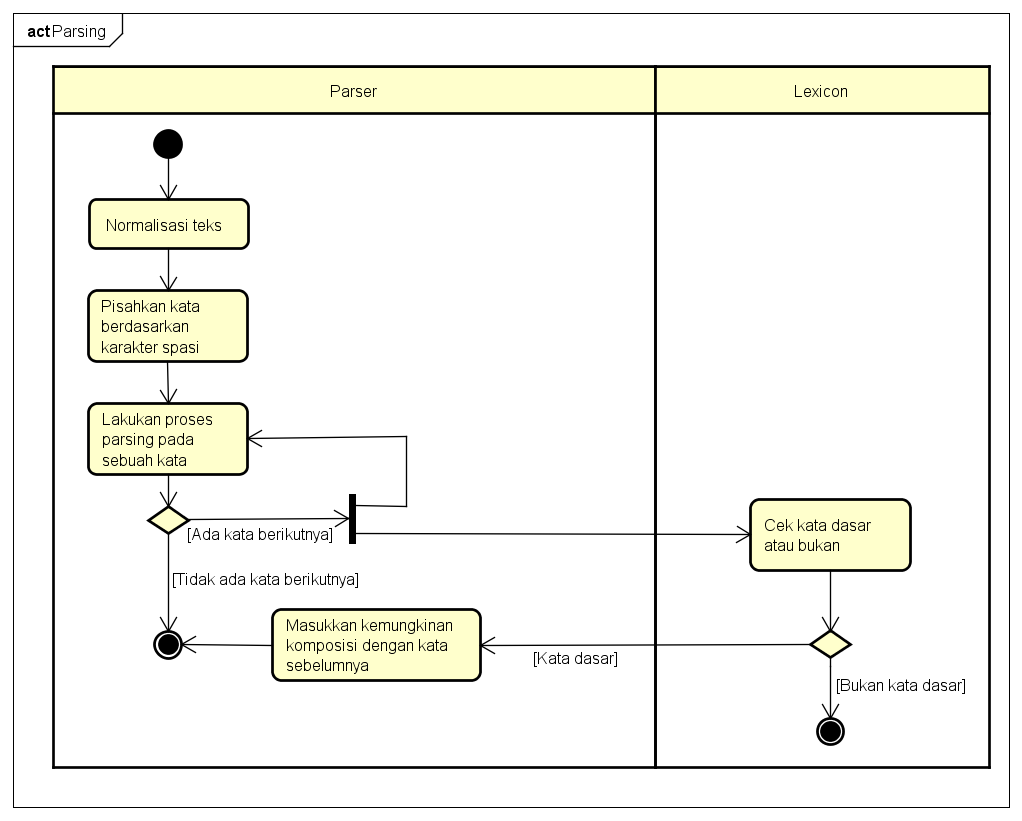
\includegraphics[scale=0.45]{Gambar/gambar-diagram-aktivitas-olah-masukan}
\caption{Diagram aktivitas proses mengolah teks masukan} 
\label{gambar-diagram-aktivitas-olah-masukan}
\end{figure}

Gambar \ref{gambar-diagram-aktivitas-satu-kata} berikut adalah diagram aktivitas yang dibuat untuk proses parsing pada sebuah kata.

\begin{figure}[H]
\centering
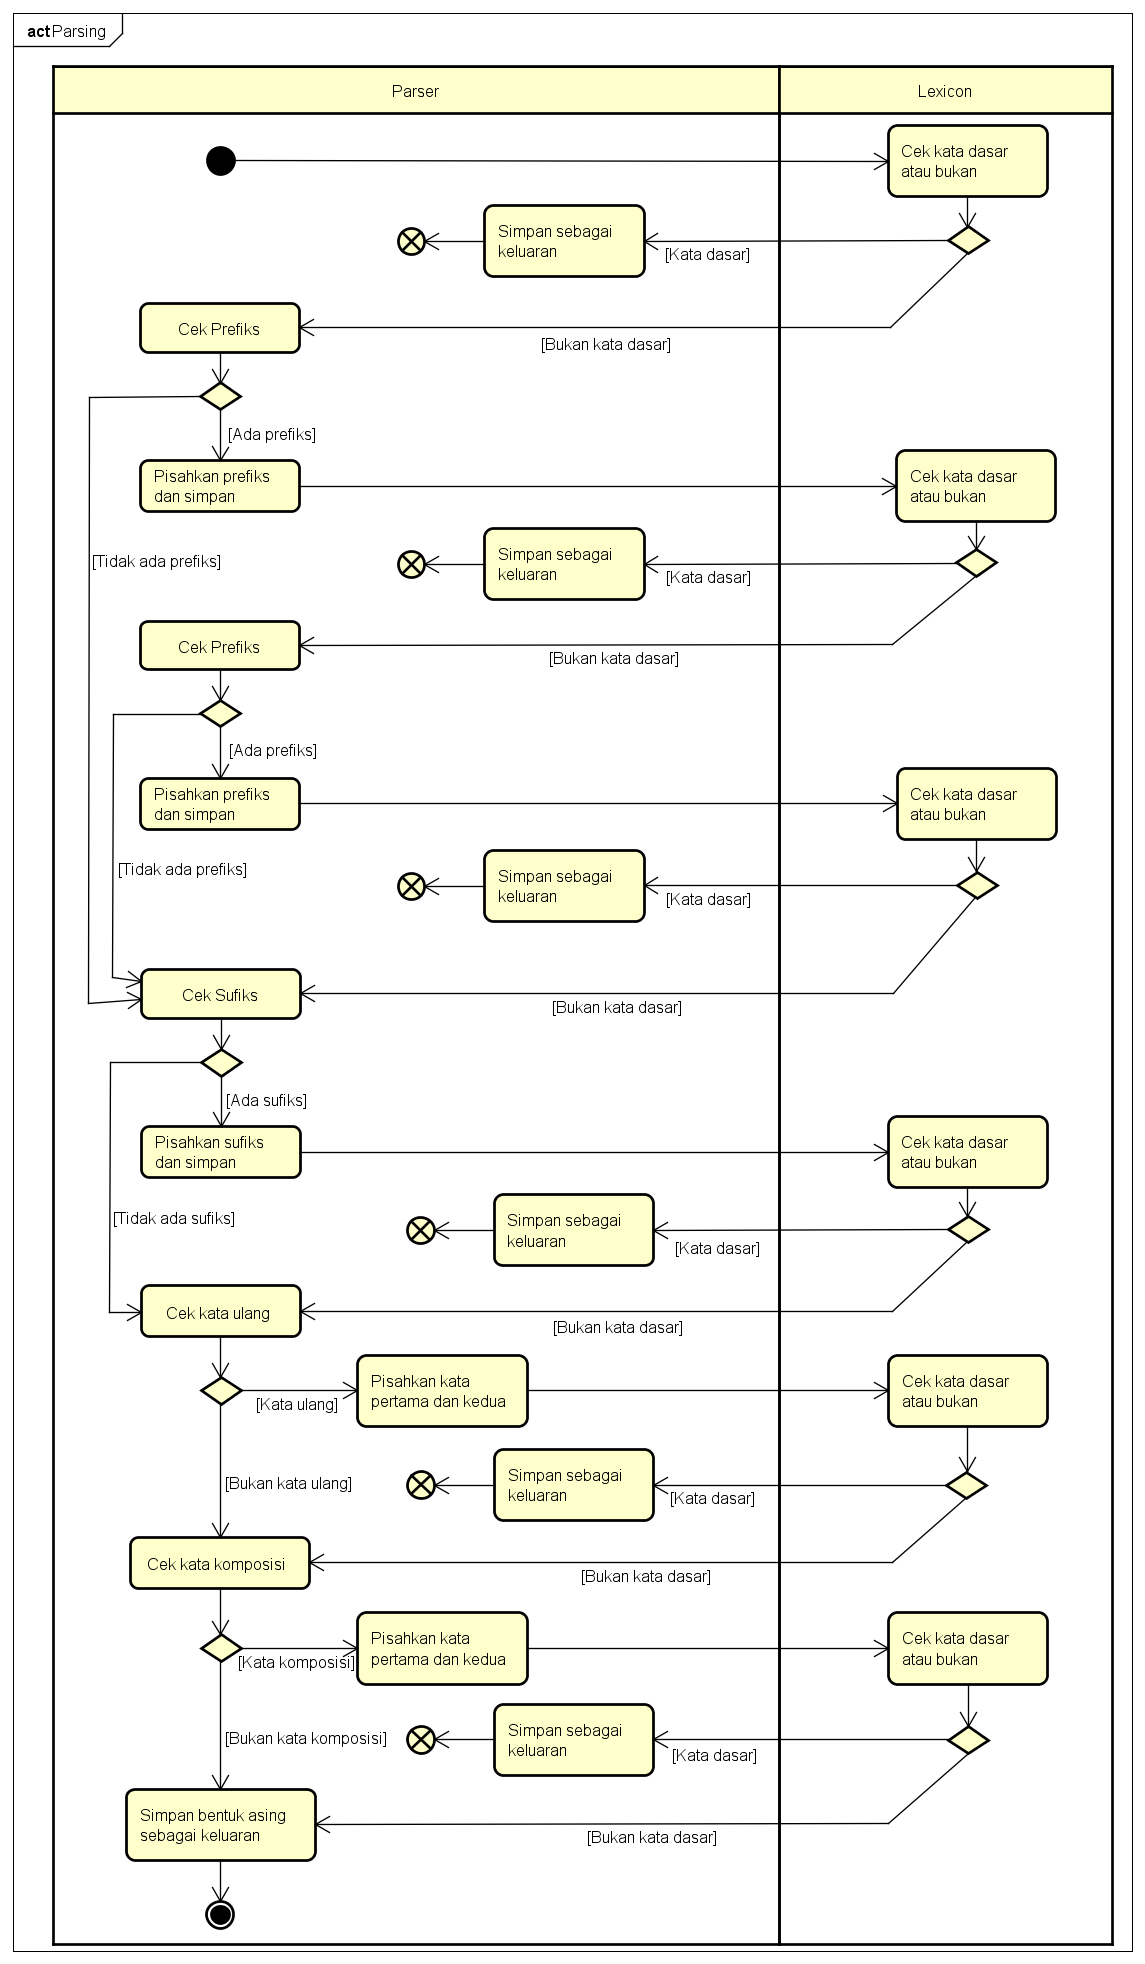
\includegraphics[scale=0.4]{Gambar/gambar-diagram-aktivitas-satu-kata}
\caption{Diagram aktivitas proses parsing pada sebuah kata} 
\label{gambar-diagram-aktivitas-satu-kata}
\end{figure}